%---------------------------------------------------------------------
\section{Resultados das simula��es}

Simula��o utilizando \HI{\texttt{Matlab/Simulink}}.

\subsection{Simula��o \#1}

\bigskip%
Par�metros e condi��es iniciais  :
%
\begin{align*}
  a_p &= -2\,,  &  y_p(0) &= 0\,, & \theta(0) &= 0\,, \\
  a_m &= 1\,,   &  y_m(0) &= 0\,, & \gamma &= 10,\ 100\,, \\
  r &= 1\,.
\end{align*}

\bigskip%
\begin{figure}[H]
  \centering
  \includegraphics[width=12cm]{figs/fig01d.eps} \\[2mm]
  \caption{Diagrama $e_0 \times \tilde{\theta}$.
  \hfill (Script: \HI{\tt simu01.m}) }
\end{figure}

\newpage%
%---------------------------------------------------------------------
\begin{figure}[H]
  \centering
  \includegraphics[width=12cm]{figs/fig01c.eps} \\[2mm]
  \includegraphics[width=12cm]{figs/fig01a.eps} \\[2mm]
  \includegraphics[width=12cm]{figs/fig01b.eps} \\[2mm]
  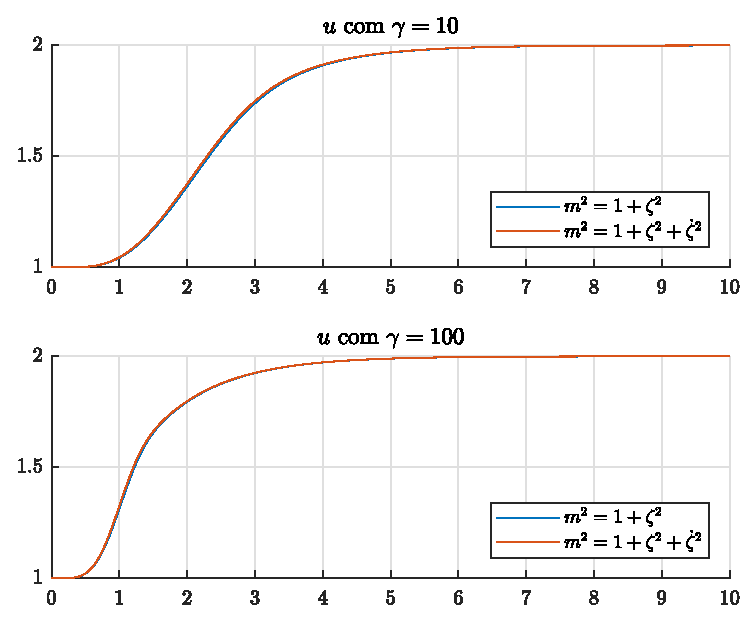
\includegraphics[width=12cm]{figs/fig01e.eps} \\[2mm]
  \caption{Resultado da simula��o com algoritmo Gradiente normalizado.
  \hfill (Script: \HI{\tt simu01.m}) }
\end{figure}


\newpage%
%---------------------------------------------------------------------
\subsection{Simula��o \#2}

\bigskip%
Par�metros e condi��es iniciais  :
%
\begin{align*}
  a_p &= -2\,,  &  y_p(0) &= \HI{2}\,, & \theta(0) &= 0\,, \\
  a_m &= 1\,,   &  y_m(0) &= 0\,, & \gamma &= 2,\ 100\,, \\
  r &= 1\,.
\end{align*}

\bigskip%
\begin{figure}[H]
  \centering
  \includegraphics[width=12cm]{figs/fig02d.eps} \\[2mm]
  \caption{Diagrama $e_0 \times \tilde{\theta}$.
  \hfill (Script: \HI{\tt simu02.m}) }
\end{figure}

\newpage%
%---------------------------------------------------------------------
\begin{figure}[H]
  \centering
  \includegraphics[width=12cm]{figs/fig02c.eps} \\[2mm]
  \includegraphics[width=12cm]{figs/fig02a.eps} \\[2mm]
  \includegraphics[width=12cm]{figs/fig02b.eps} \\[2mm]
  \includegraphics[width=12cm]{figs/fig02e.eps} \\[2mm]
  \caption{Resultado da simula��o com algoritmo Gradiente normalizado.
  \hfill (Script: \HI{\tt simu02.m}) }
\end{figure}

\newpage%
%---------------------------------------------------------------------
\subsection{Simula��o \#3}

\bigskip%
Par�metros e condi��es iniciais  :
%
\begin{align*}
  a_p &= -2\,,  &  y_p(0) &= \HI{10}\,, & \theta(0) &= 0\,, \\
  a_m &= 1\,,   &  y_m(0) &= 0\,, & \gamma &= 2,\ 100\,, \\
  r &= 1\,.
\end{align*}

\bigskip%
\begin{figure}[H]
  \centering
  \includegraphics[width=12cm]{figs/fig03d.eps} \\[2mm]
  \caption{Diagrama $e_0 \times \tilde{\theta}$.
  \hfill (Script: \HI{\tt simu03.m}) }
\end{figure}

\newpage%
%---------------------------------------------------------------------
\begin{figure}[H]
  \centering
  \includegraphics[width=12cm]{figs/fig03c.eps} \\[2mm]
  \includegraphics[width=12cm]{figs/fig03a.eps} \\[2mm]
  \includegraphics[width=12cm]{figs/fig03b.eps} \\[2mm]
  \includegraphics[width=12cm]{figs/fig03e.eps} \\[2mm]
  \caption{Resultado da simula��o com algoritmo Gradiente normalizado.
  \hfill (Script: \HI{\tt simu03.m}) }
\end{figure}